% !TeX spellcheck = fr_FR
\section{Développement firmware}
Dans cette section, nous allons décrire et expliquer le processus de programmation du code qui a été implémenté dans le microcontrôleur PIC32MX130F256D.
Le processus de programmation du code dans le PIC32MX130F256D comprend plusieurs étapes. Tout d'abord, il est nécessaire de disposer d'un environnement de développement intégré (IDE) adapté à ce microcontrôleur, tel que MPLAB X IDE. Cet IDE est équipé de l'environnement Harmony, qui permet l'utilisation d'un configurateur graphique pour les différentes bibliothèques du PIC.

\subsection{Configuration des PINs dans Harmony}
{
	\begin{figure}[h]
		\centering
		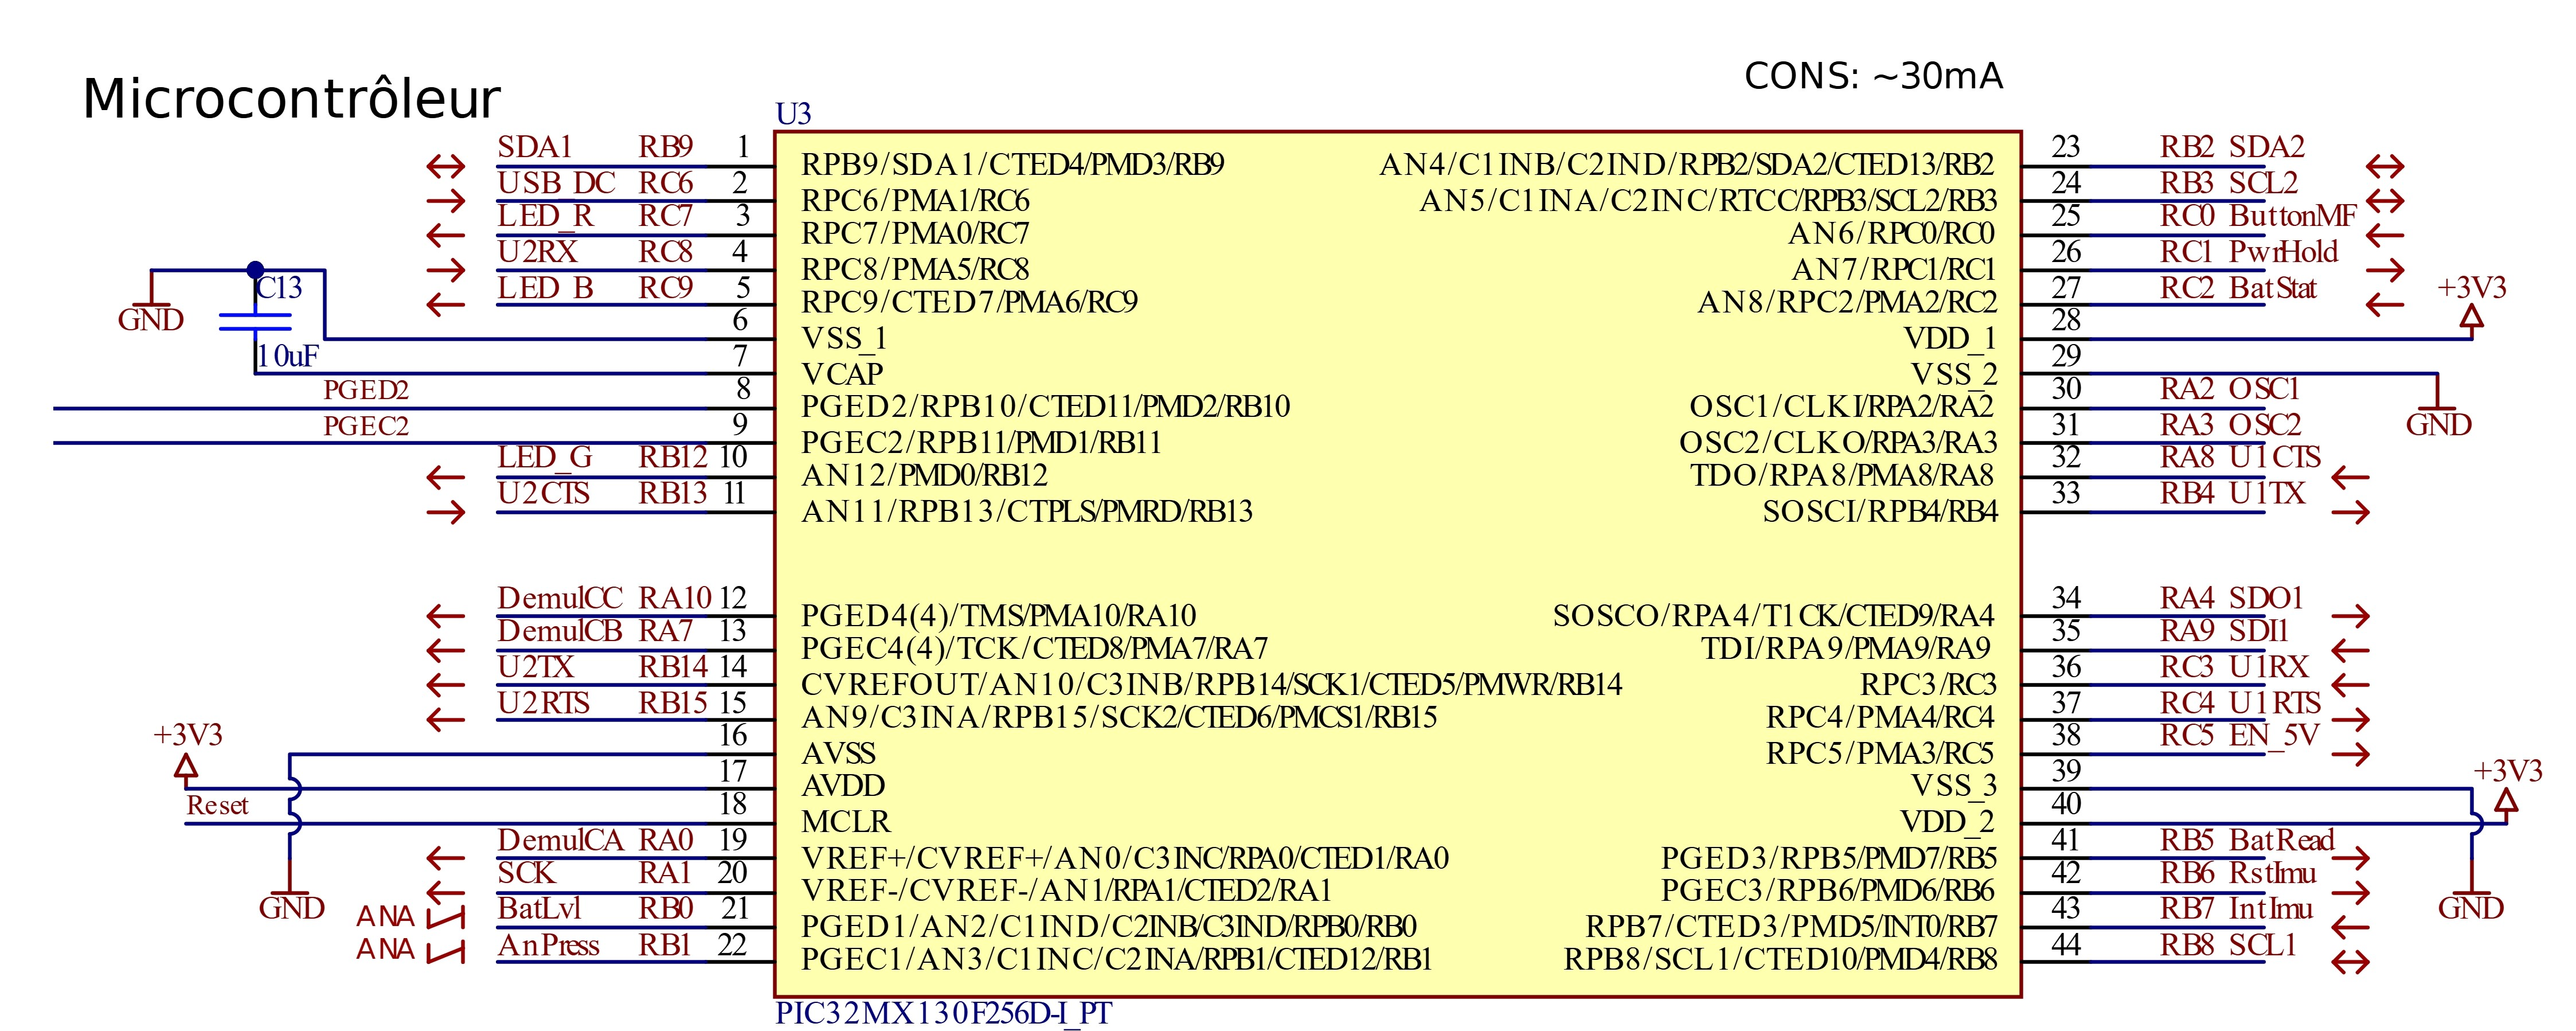
\includegraphics[width=.9\textwidth]{Figures/Dev-SOFT/MCU-Altium}
		\caption{Pinning réelles dans altium designer}
		\label{fig:mcu-altium}
	\end{figure}
	\begin{figure}[h]
		\centering
		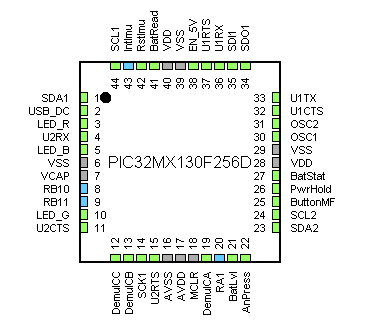
\includegraphics[width=0.5\textwidth]{Figures/Dev-SOFT/MCU-Harmony}
		\caption{Pinning dans Harmony}
		\label{fig:mcu-harmony}
	\end{figure}
	
	On peut constater que la PIN 20 (SCK) est en haute impédance dans Harmony, tandis que la PIN 14, qui était supposée être \textit{U2TX}, est maintenant configurée en tant que SCK. Cela est dû à une erreur : SCK ne peut être assigné qu'à la PIN 14. Par conséquent, il a été nécessaire d'ajouter un fil externe pour relier la PIN 14 à la PIN 20, ce qui a entraîné la perte de la communication USB sur l'UART2. Cette modification sera expliquée en détail ultérieurement.
	
	
}

\subsection{Configuration des périphériques dans Harmony}
{
	\subsubsection{Timers} 
	
	Deux timers seront utilisés, l'un pour mesurer des attentes en ms et l'autre moins rapide, pour les diverses actions du programmes, avec une interruptions chaque 10ms.
	\begin{table}[h]
		\centering
		\begin{tabular}{|l|l|}
			\hline
			Timer & Temps voulu \\
			\hline
			Timer 1 & 1ms \\
			\hline
			Timer 2 & 10ms \\
			\hline
		\end{tabular}
	\end{table}

	La fréquence de l'horloge système a été augmentée à 48 MHz dans le but d'accélérer l'ensemble du système, étant donné qu'il implique de nombreuses communications nécessitant des opérations rapides, que ce soit pour la préparation des tampons de données ou les divers calculs.
	
	\begin{figure}[h]
		\centering
		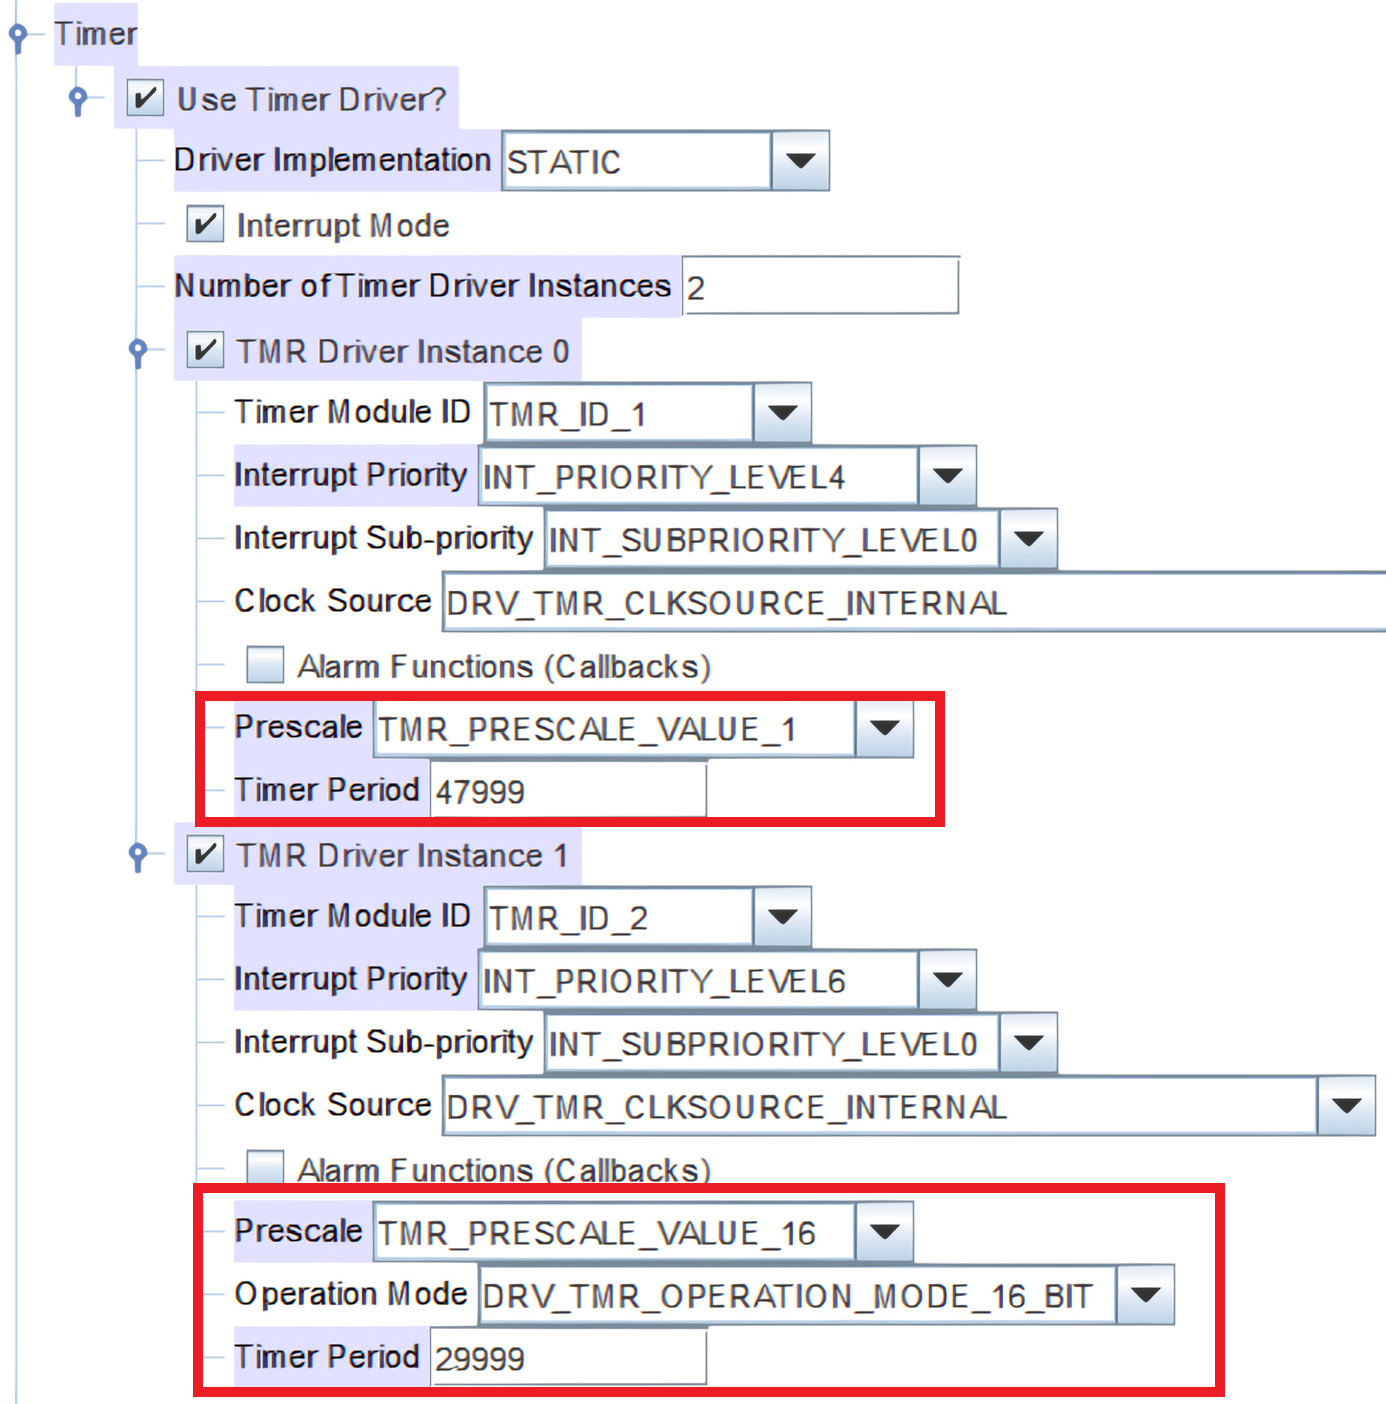
\includegraphics[width=0.55\linewidth]{Figures/Dev-SOFT/Timer_config}
		\caption{Configuration dans harmony}
		\label{fig:timerconfig}
	\end{figure}

	\begin{figure}[h]
		\centering
		\begin{subfigure}[b]{0.45\textwidth}
			\centering
			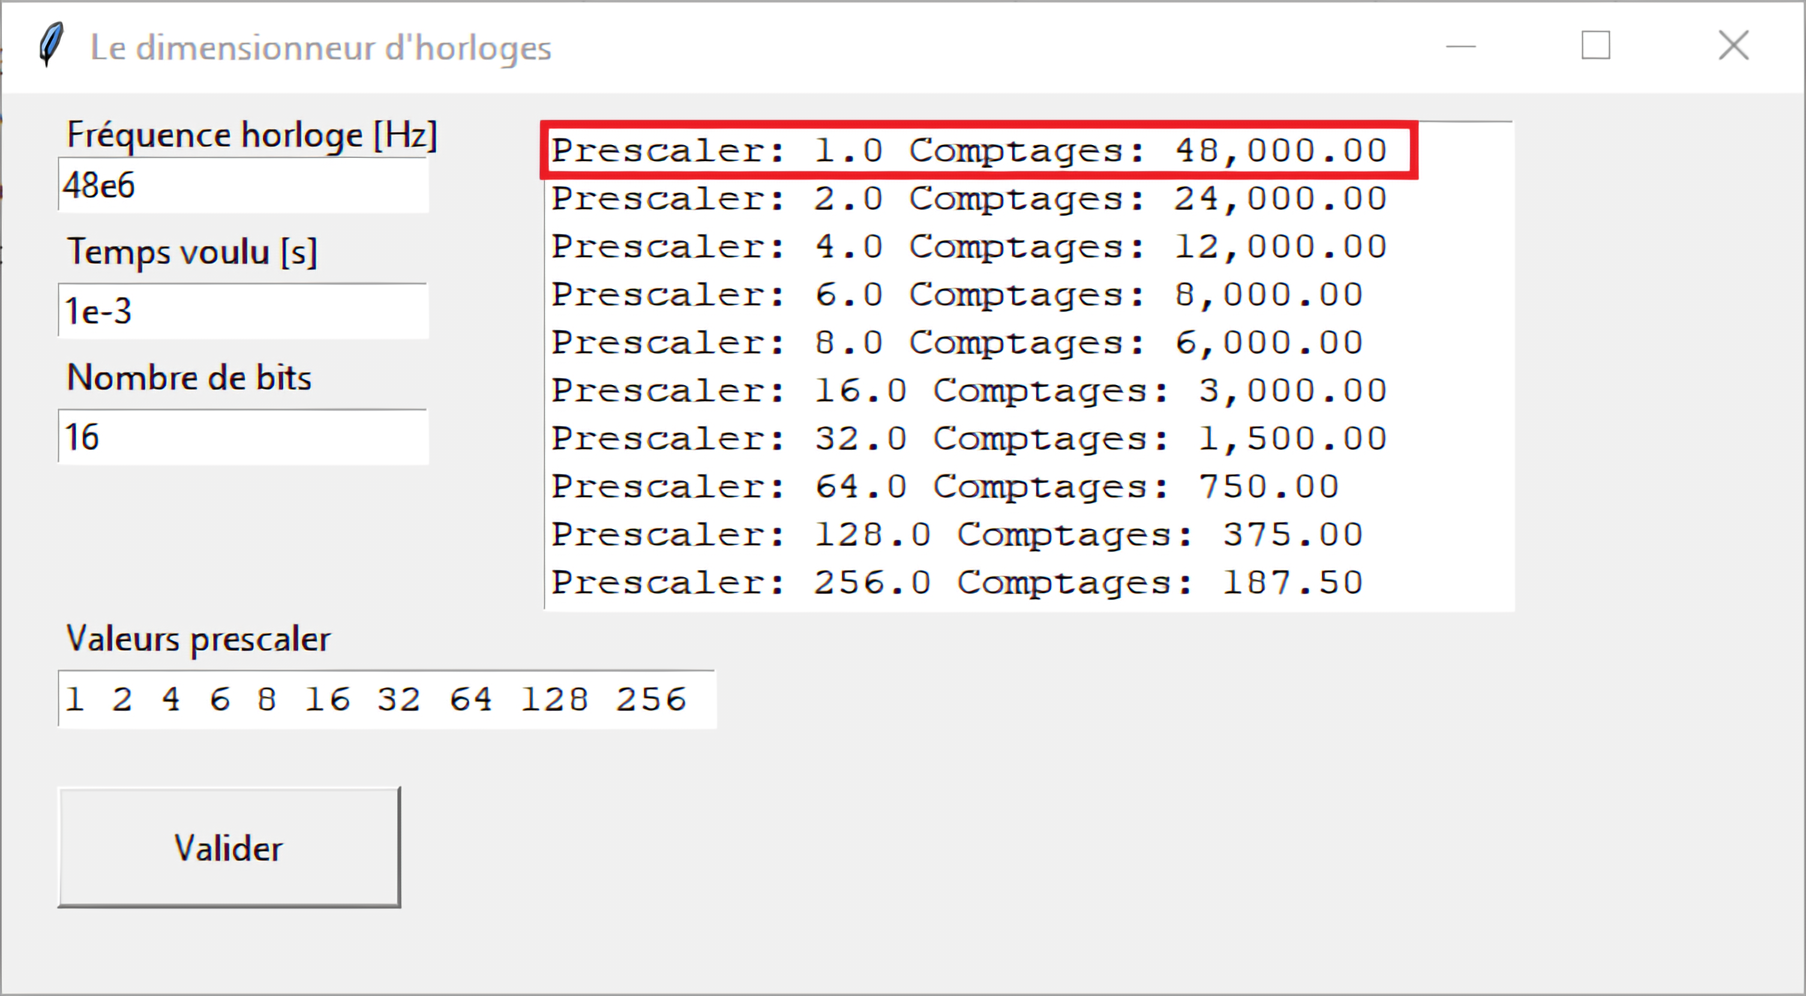
\includegraphics[width=\textwidth]{Figures/Dev-SOFT/Timer1ms}
			\caption{Timer 1, Dimensionnement pour 1ms}
			\label{fig:timer1ms}
		\end{subfigure}
		\hfill
		\begin{subfigure}[b]{0.45\textwidth}
			\centering
			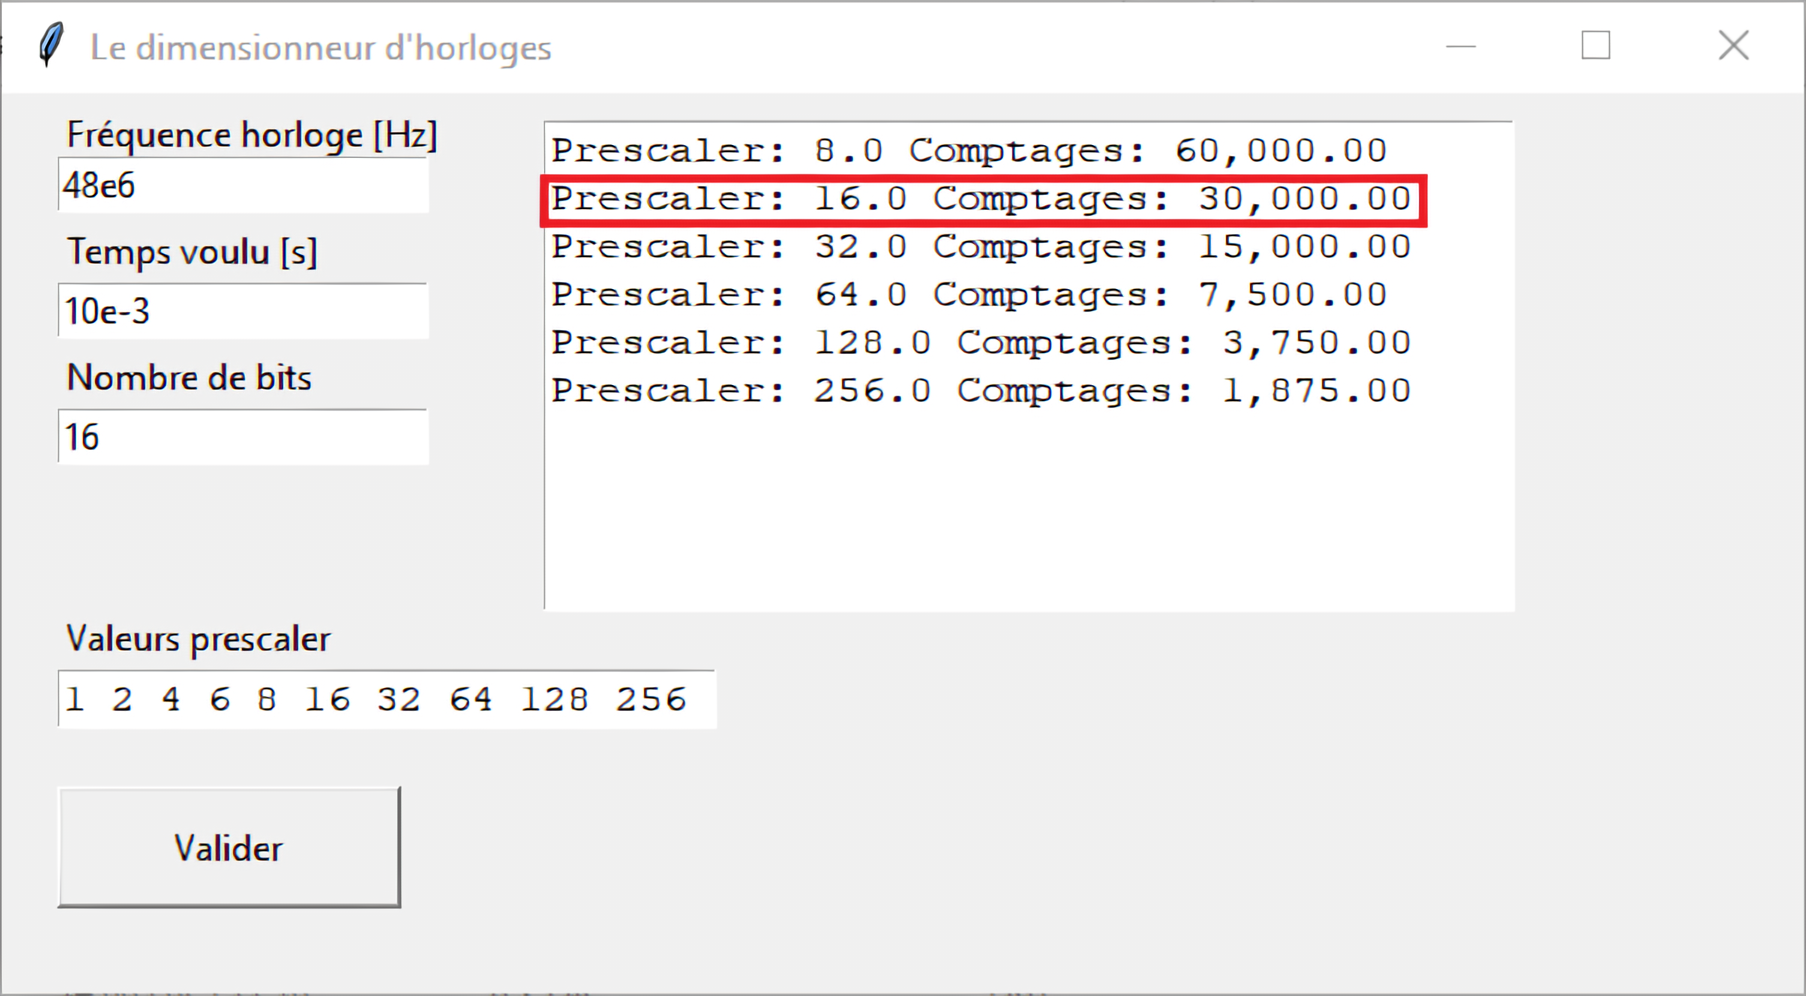
\includegraphics[width=\textwidth]{Figures/Dev-SOFT/Timer10ms}
			\caption{Timer 2, Dimensionnement pour 10ms}
			\label{fig:timer10ms}
		\end{subfigure}
		\hfill
		\caption{Application timer développée par l'auteur}
		\label{fig:appTimer}
	\end{figure}

	\clearpage

	\subsubsection{USART} \label{ssec:Usart}
	Dans le but de vérifier les données de mesure en temps réel et de faciliter le débogage, une communication sérielle UART a été mise en place. Pour cela, le périphérique UART1, initialement prévu pour le slot mikroe, a été utilisé. Un module USB-to-TTL externe sera utilisé pour lire les données via Putty sur un ordinateur.
	
	\begin{figure}[h]
		\centering
		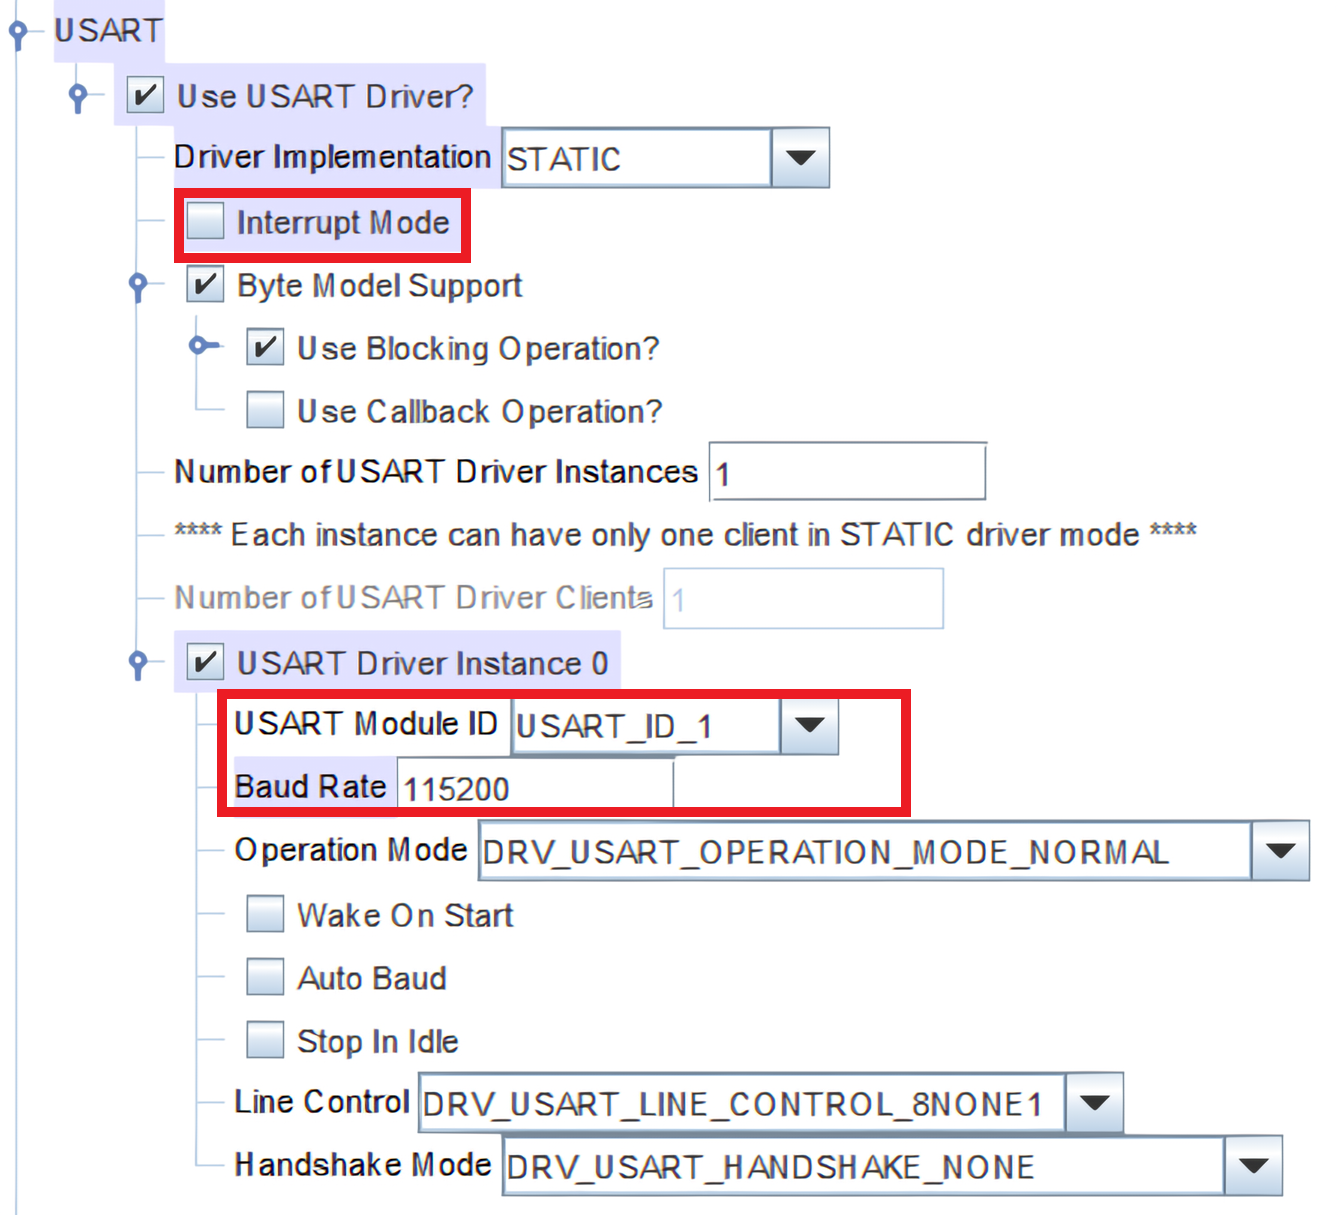
\includegraphics[width=0.7\linewidth]{Figures/Dev-SOFT/ConfigUart}
		\caption{Configuration UART}
		\label{fig:configuart}
	\end{figure}
	
	
	Nous pouvons constater sur la figure \ref{fig:configuart} que l'UART est configuré sans interruption à un bauderate de 115200.

	\subsubsection{Carte SD - SPI} 
	{
	L'utilisation du SPI a été optimisée en choisissant une fréquence de 5 MHz afin de réduire le temps d'exécution sur le microcontrôleur, compte tenu du grand nombre de trames nécessaires pour les opérations FAT. Cependant, j'ai rencontré un problème lié à la clock du SPI. En raison de la vitesse élevée et des modifications que j'ai dû apporter, la clock interfère inutilement avec le FTDI, et un fil relie SCK et U2TX, créant ainsi une inductance parasite. Pour résoudre ce problème, j'ai ajouté un condensateur de \textbf{33pF} entre SCK et GND pour stabiliser la communication. Vous pouvez consulter la configuration Harmony de la carte SD sur la figure \ref{fig:configsdspi}.
	\clearpage
	\begin{figure}[h]
		\centering
		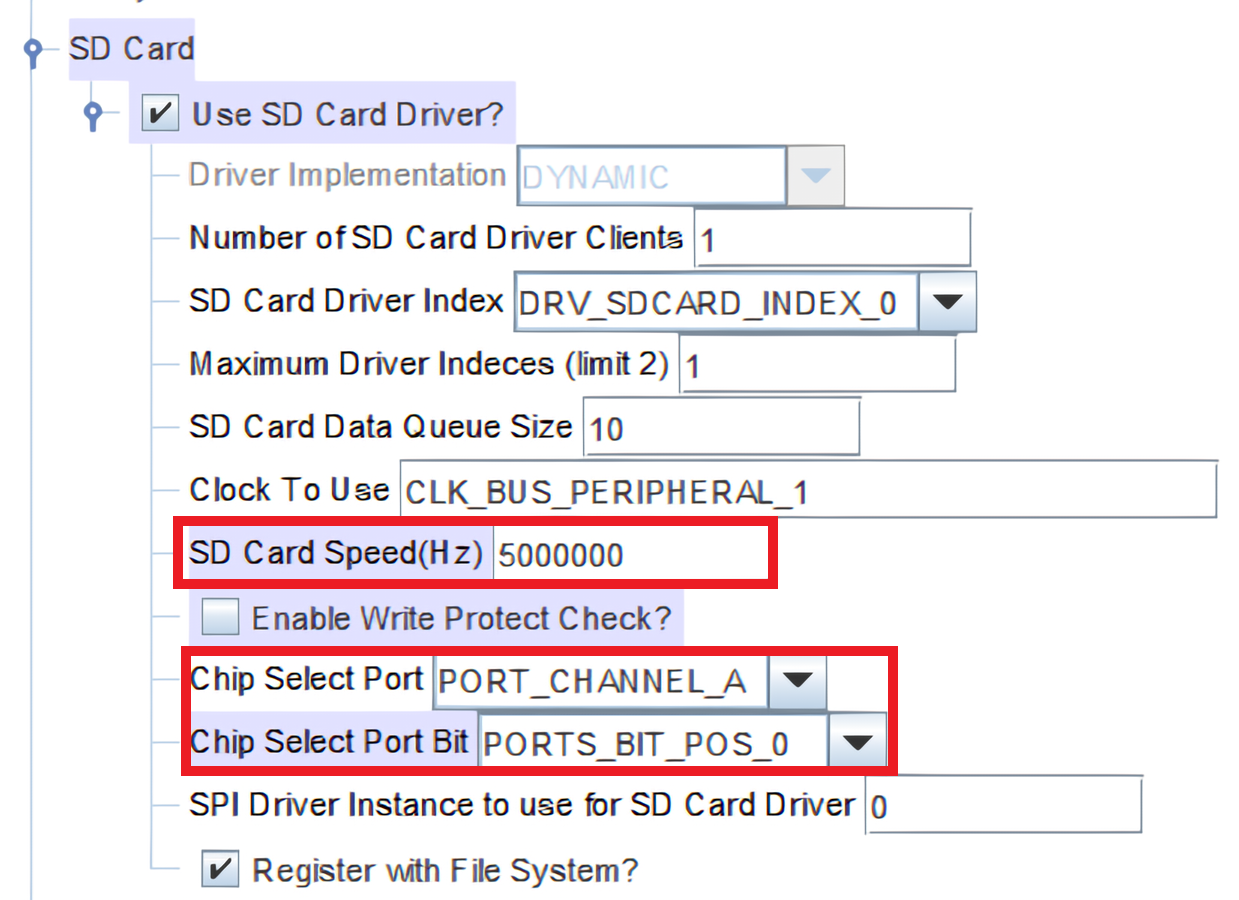
\includegraphics[width=0.7\linewidth]{Figures/Dev-SOFT/ConfigSD_SPI}
		\caption{Configuration du SPI}
		\label{fig:configsdspi}
	\end{figure}
	}

	\subsection{Code}
	Je vais dans cette section décrire le code du projet. Voici la hiérarchie des fichier du projet :
	\begin{figure}[h]
		\centering
		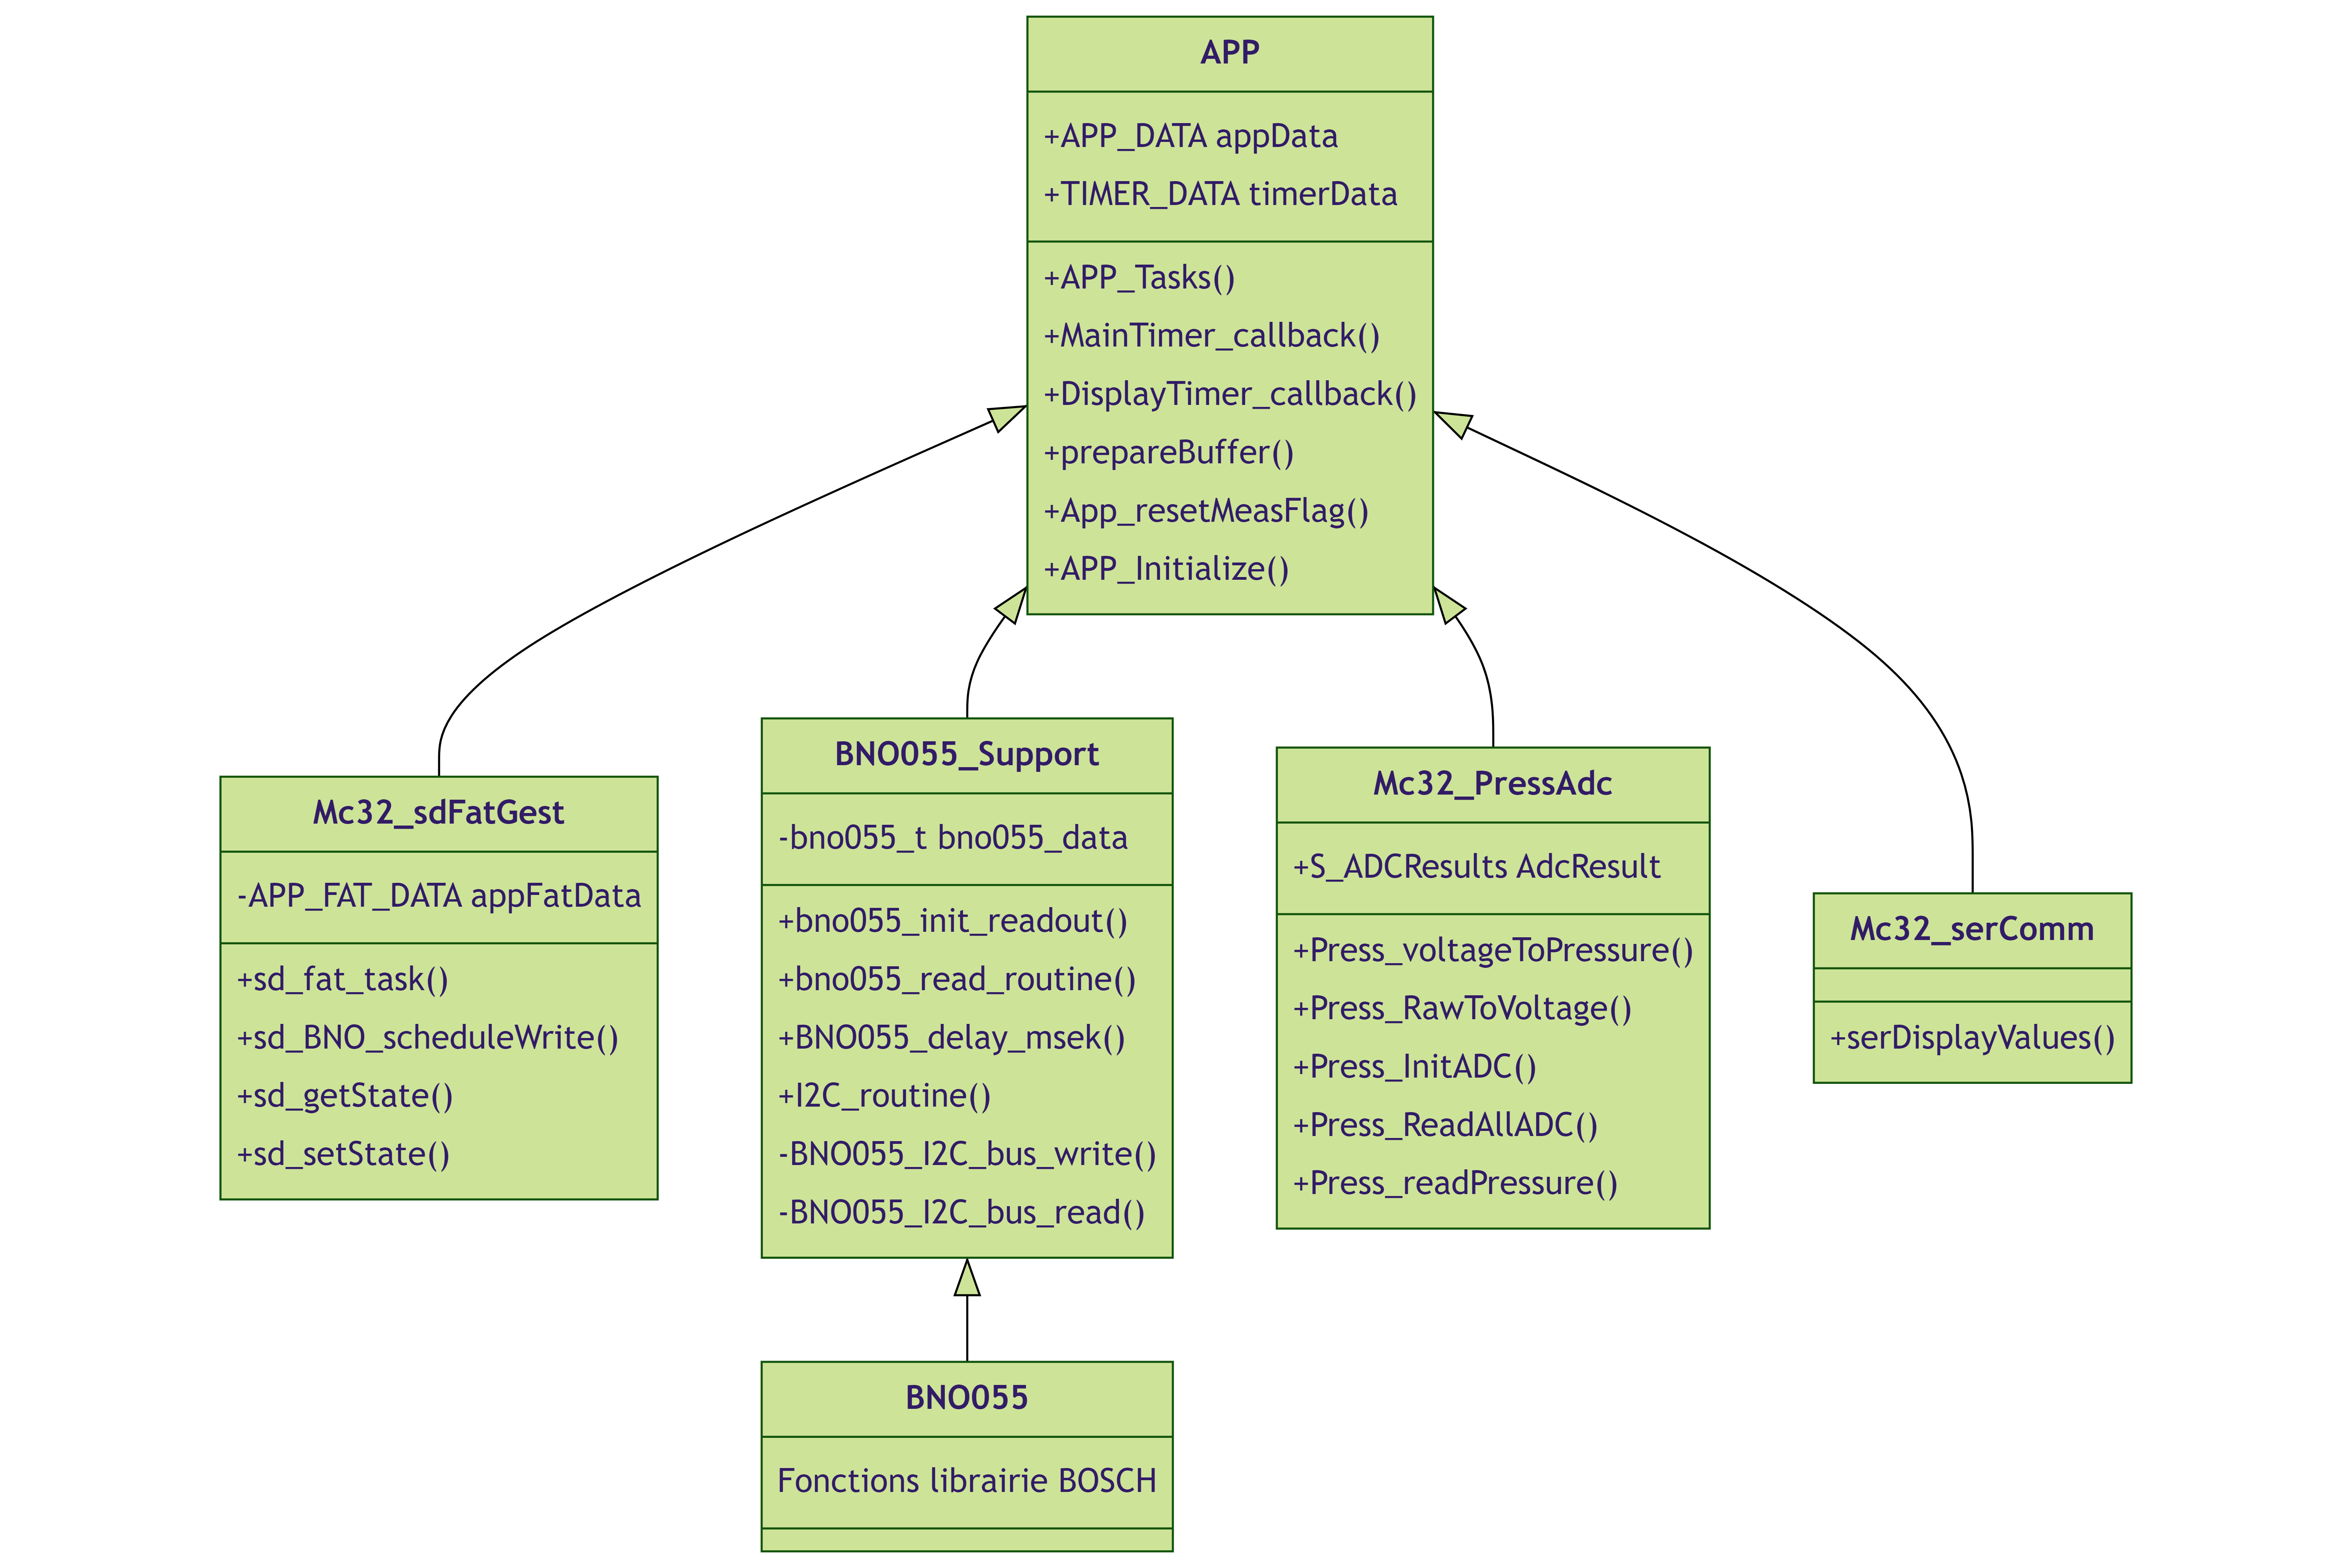
\includegraphics[width=0.79\linewidth]{Figures/Dev-SOFT/ClassesCode}
		\caption{Hiérarchie des fichiers du projet}
		\label{fig:classescode}
	\end{figure}
	
	\clearpage	
	
	\subsubsection{Callbacks}
	{
	Chacun des timers appelle dans leur interruption une fonction appartenant au fichier \textit{app.c}, qui contient les actions définies pour chaque intervalle de temps spécifique. On peut visualiser cela sur le diagramme présenté dans la figure \ref{fig:callbacks}.
	
	\begin{figure}[h!]
		\centering
		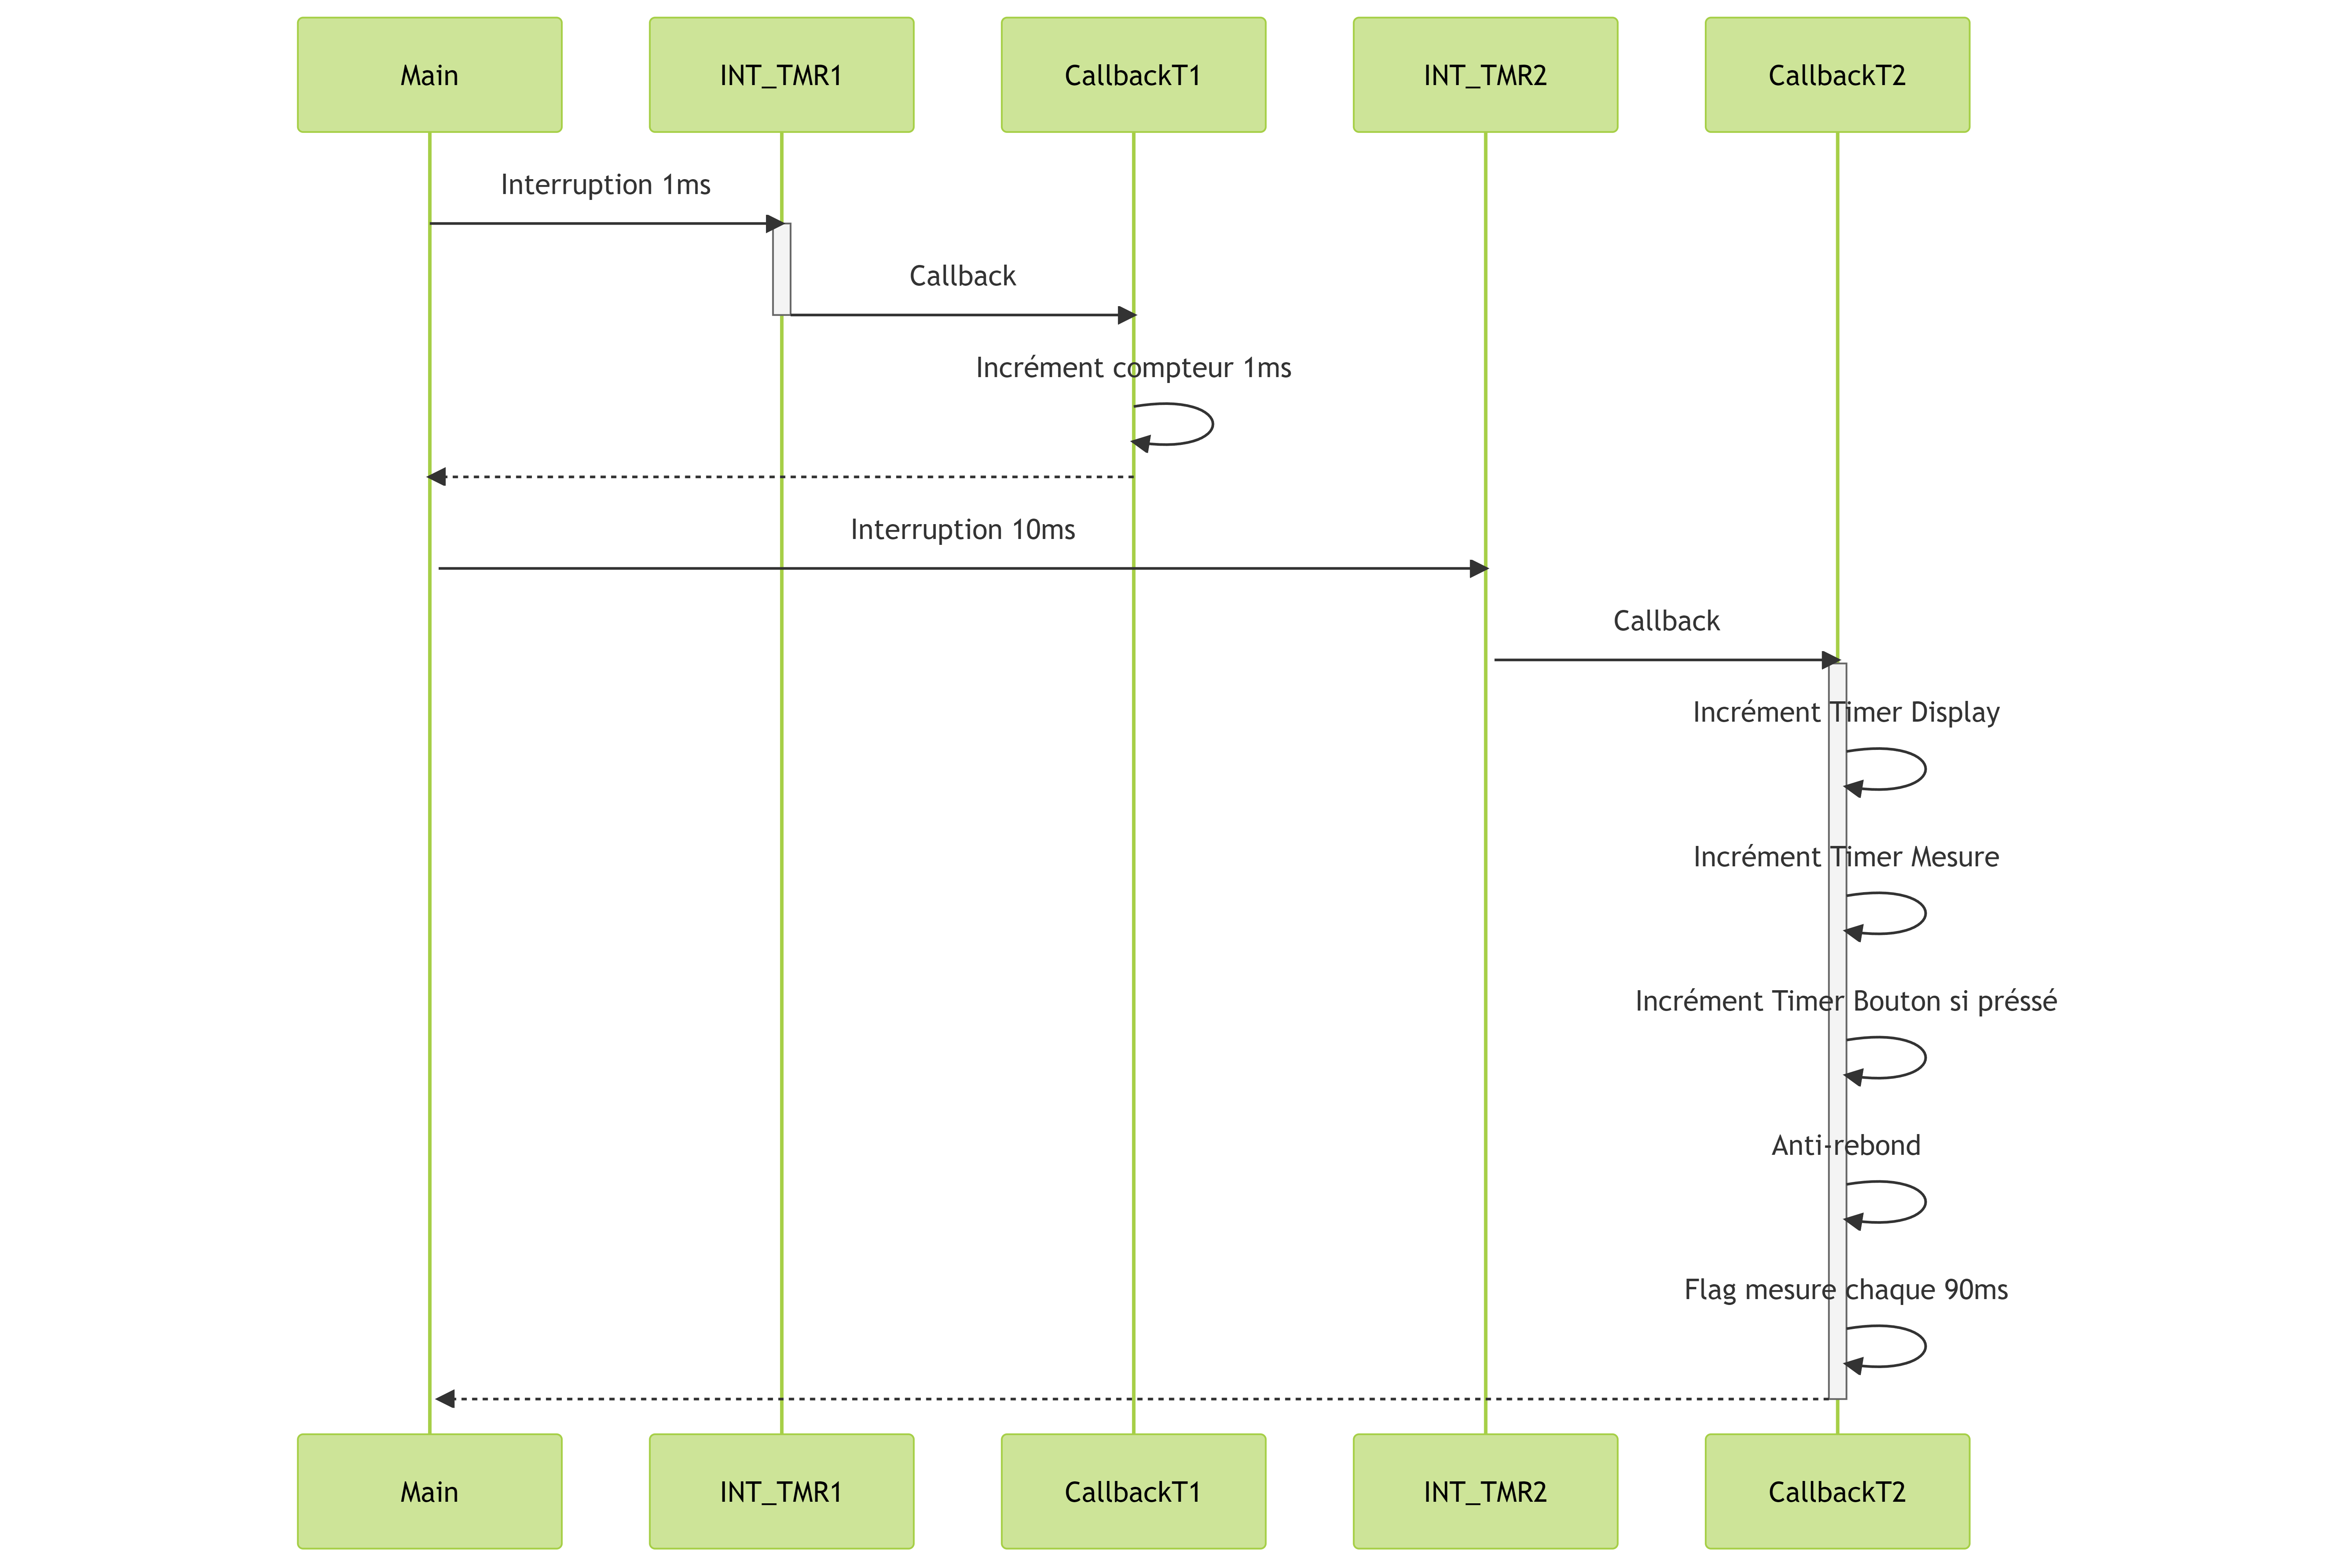
\includegraphics[width=1\textwidth]{Figures/Dev-SOFT/Callbacks}
		\caption{Interactions des interruptions et des callbacks}
		\label{fig:callbacks}
	\end{figure}

	Les callbacks en C offrent flexibilité, extensibilité et réutilisabilité. Ils permettent d'ajuster dynamiquement le comportement du programme, d'étendre les fonctionnalités et de réutiliser le code. Les callbacks favorisent également l'encapsulation et la personnalisation, améliorant ainsi la modularité et la maintenance du code.	
	}
	
	\clearpage
	\subsubsection{Centrale inertielle BNO055}
	Pour ce qui est de la centrale inertielle BNO055, j'ai utilisé la bibliothèque de BOSCH \footnote{\href{https://github.com/BoschSensortec/BNO055_driver}{Bibliothèque du fabricant}}. Je l'ai configurée en 32 bits et j'ai créé les fonctions de bas niveau (i2c) en établissant le lien avec la bibliothèque BOSCH. Tout cela a été fait dans le fichier BNO055\_support.c.
	
	Pour faire le lien entre la bibliothèque de haut niveau et la bibliothèque de bas niveau, j'ai utilisé un pointeur de fonction présent dans la structure de données du BNO, comme illustré dans le listing \ref{lst:lienPointeur}.
	
\begin{lstlisting}[frame=single, label={lst:lienPointeur}, language=C, caption={Code lien pointeur de fonction}, captionpos=b]
s8 I2C_routine(void)
{
	bno055.bus_write = BNO055_I2C_bus_write;
	bno055.bus_read = BNO055_I2C_bus_read;
	bno055.delay_msec = BNO055_delay_msek;
	bno055.dev_addr = BNO055_I2C_ADDR1;
	return BNO055_INIT_VALUE;
}
\end{lstlisting}
\begin{lstlisting}[frame=single, language=C, caption={Code écriture i2c au BNO055}, captionpos=b, breaklines=true]
s8 BNO055_I2C_bus_write(u8 dev_addr, u8 reg_addr, u8 *reg_data, u8 cnt)
{
	s8 BNO055_iERROR = BNO055_INIT_VALUE;
	u8 array[I2C_BUFFER_LEN];
	u8 stringpos = BNO055_INIT_VALUE;
	array[BNO055_INIT_VALUE] = reg_addr;
	
	i2c_start();
	BNO055_iERROR = i2c_write(dev_addr<<1);
	
	for (stringpos = BNO055_INIT_VALUE; stringpos < (cnt+BNO055_I2C_BUS_WRITE_ARRAY_INDEX); stringpos++)
	{
		BNO055_iERROR = i2c_write(array[stringpos]);
		array[stringpos + BNO055_I2C_BUS_WRITE_ARRAY_INDEX] = *(reg_data + stringpos);
	}
	
	i2c_stop();
	if(BNO055_iERROR-1 != 0)
		BNO055_iERROR = -1;
	else
		BNO055_iERROR = 0;
	return (s8)(BNO055_iERROR);
}
\end{lstlisting}
	Pour ce qui est de l'utilisation de la libraire haut-niveau bno055\_support, voici la préparation et la lecture des données : 
	
	\begin{lstlisting}[frame=single, language=C, caption={Code lecture des données par la librairie}, captionpos=b, breaklines=true]
/* BNO055 Read all important info routine */
bno055_local_data.comres = bno055_read_routine(&bno055_local_data);
/* Delta time */
bno055_local_data.d_time = timerData.TmrMeas - timerData.ltime;
/* Pressure measure */
bno055_local_data.pressure = Press_readPressure();
/* Flag measure value */
bno055_local_data.flagImportantMeas = flagMeas;
	\end{lstlisting}

	\subsubsection{Carte SD}
	La  communication de la carte SD fonctionne sous forme d'une machine d'état non-bloquante, permettant ainsi de s'adapter aux situations de la carte sans bloquer le système pour autant.
	
	\begin{figure}[h]
		\centering
		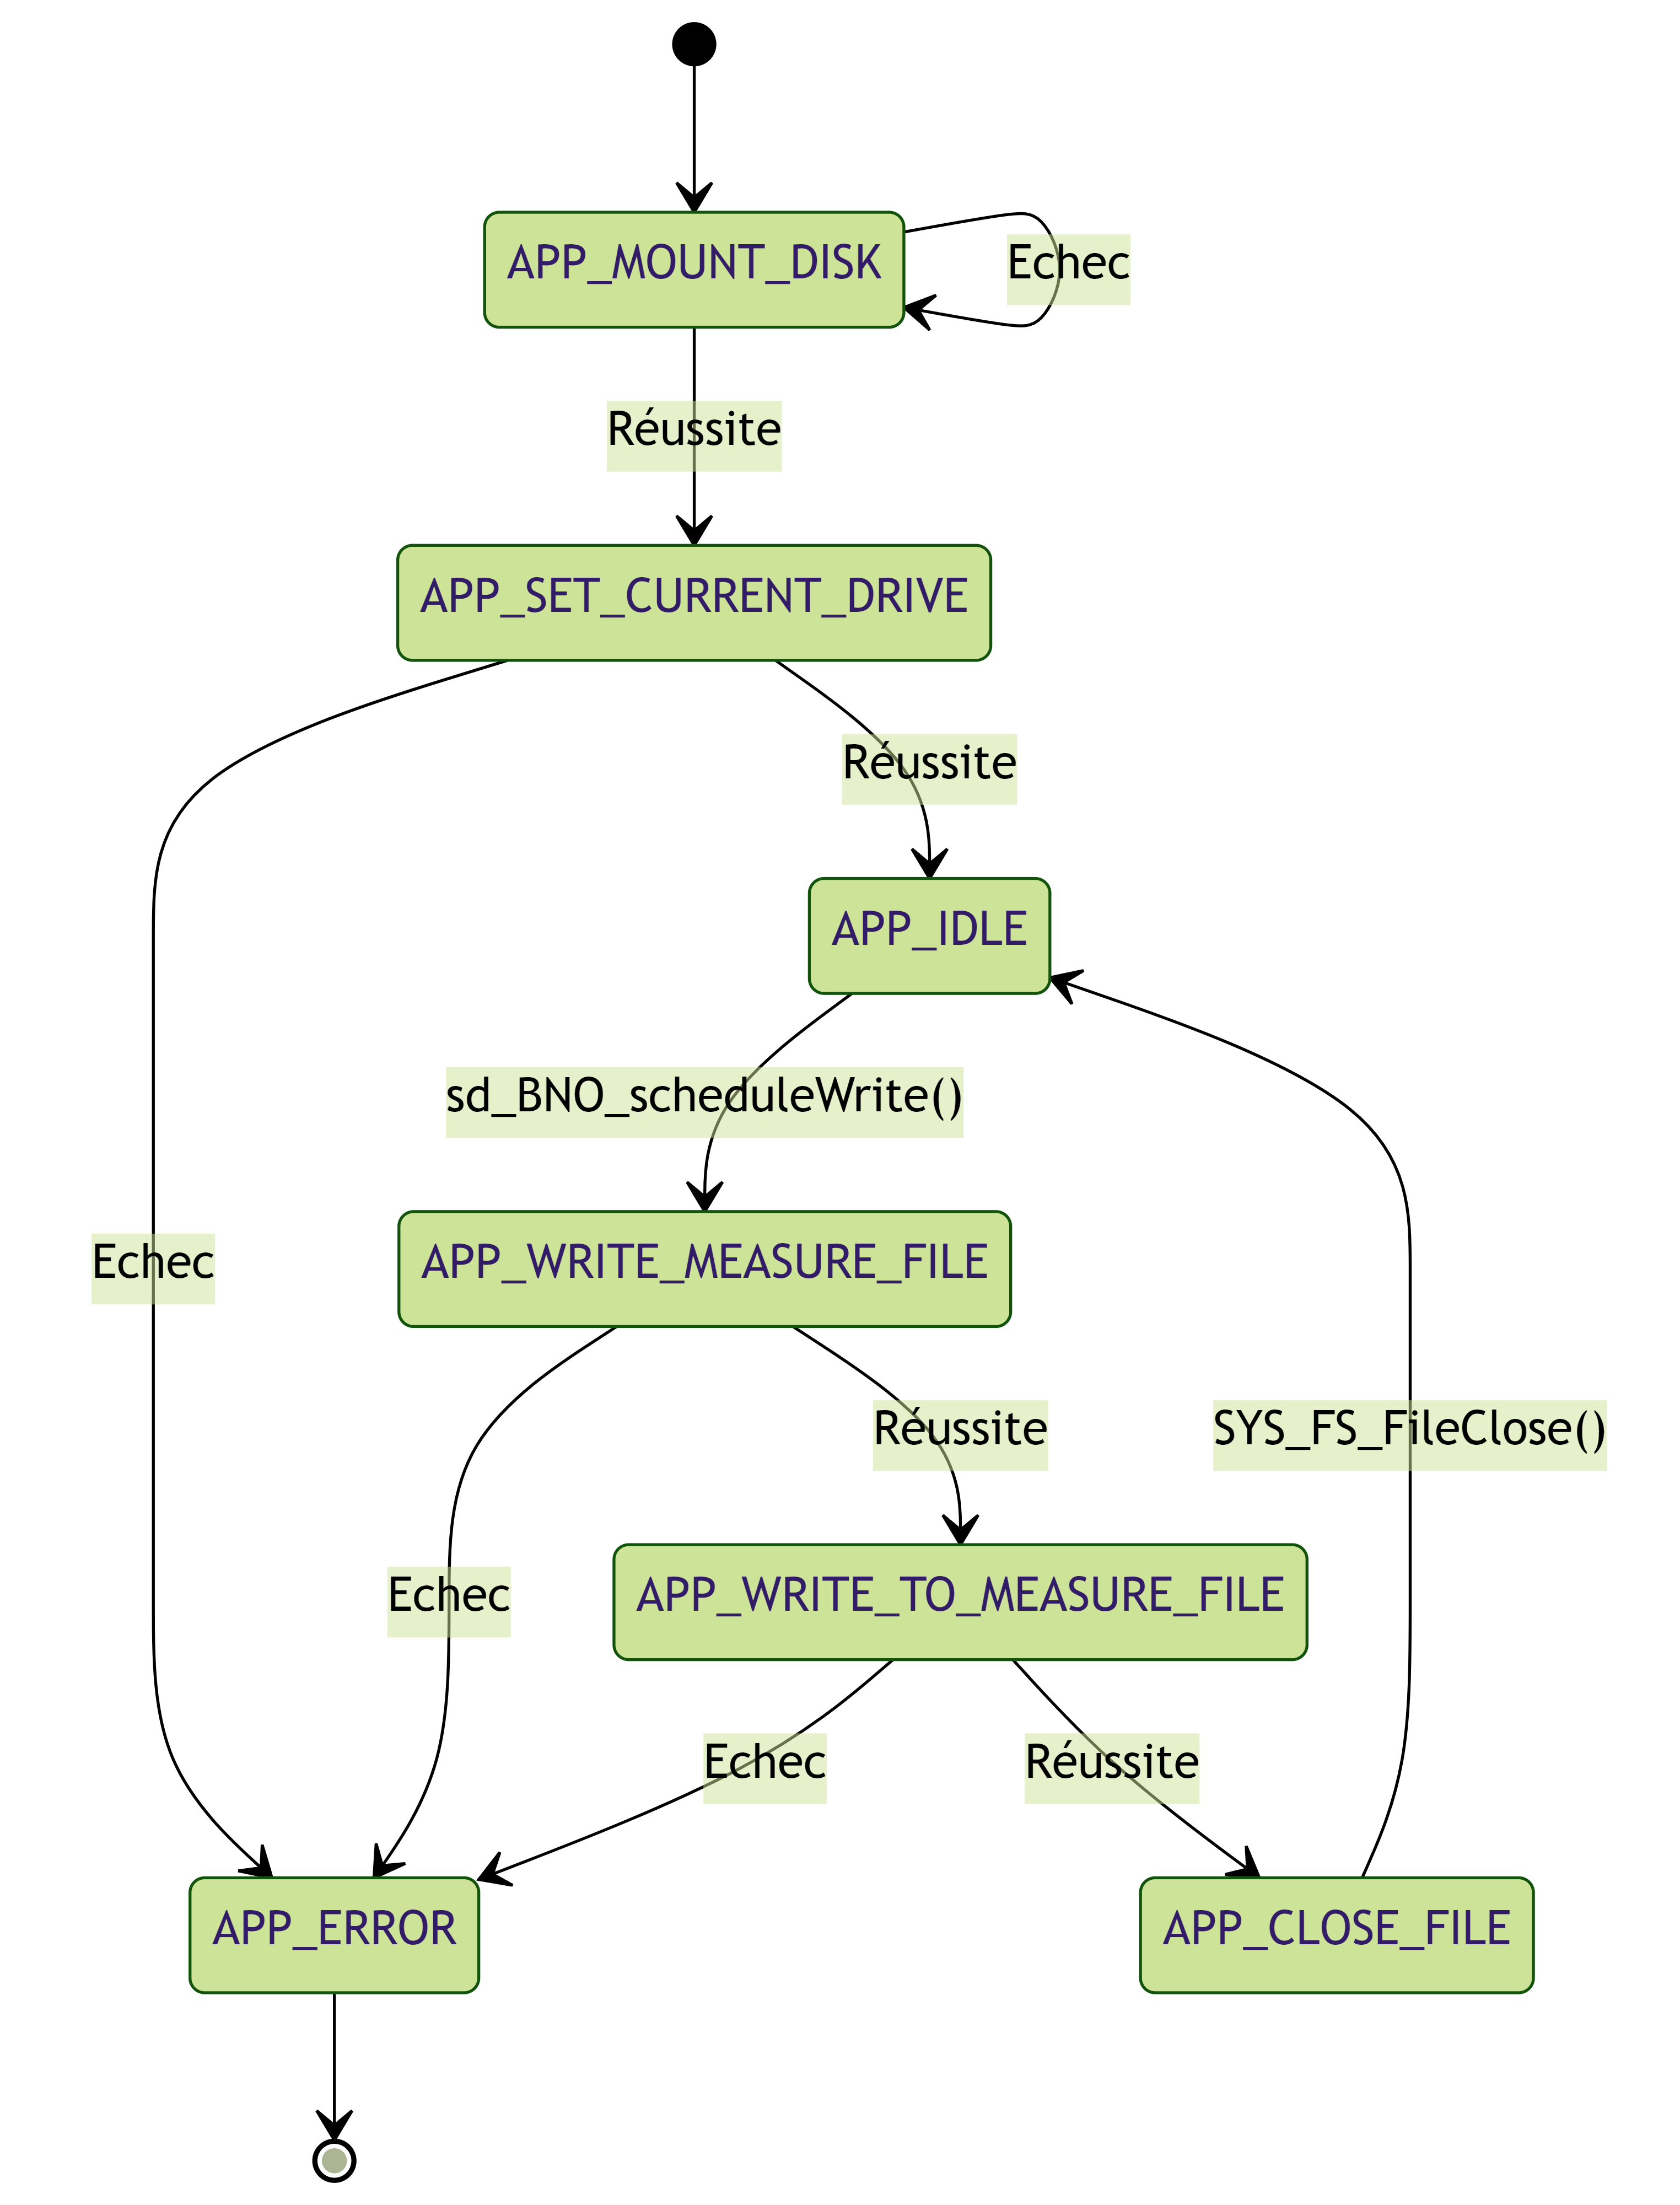
\includegraphics[width=0.6\linewidth]{Figures/Dev-SOFT/mermaid-diagram-2023-06-14-162436}
		\caption{Machine d'état de la carte SD}
		\label{fig:mermaid-diagram-2023-06-14-162436}
	\end{figure}

	\clearpage
	
	\paragraph{Planification d'une écriture}
	Afin de lancer une écriture d'un set de mesure sur la carte SD, il faut utiliser la fonction \textit{sd\_BNO\_scheduleWrite()} qui vas préparer le buffer d'écriture et modifier l'état de la carte SD : 
	\begin{lstlisting}[frame=single, language=C, caption={Lancement d'une écriture sur la carte SD}, captionpos=b, breaklines=true]
/* Write measures to sdCard */
sd_BNO_scheduleWrite(&bno055_local_data);
	\end{lstlisting}
	
	Les données sont écrite dans un fichier .CSV nommé "MESURES". La forme de la trame est la suivante :
	
	\begin{figure}[h]
		\centering
		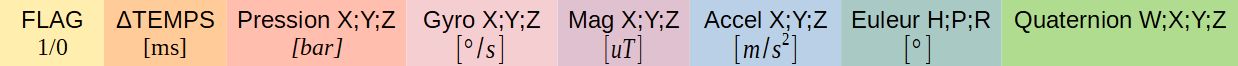
\includegraphics[width=1\textwidth]{Figures/Dev-SOFT/Trame}
		\caption{Format de la trame}
		\label{fig:trame}
	\end{figure}

	\begin{lstlisting}[frame=single, language=C, caption={Ecriture du buffer}, captionpos=b, breaklines=true]
"%d;%d0;%f;%.4f;%.4f;%.4f;%.4f;%.4f;%.4f;%.4f;%.4f;%.4f;%.4f;%.4f;%.4f;%.4f;%.4f;%.4f;%d;%d;%d;%d;"
	\end{lstlisting}
	
	\paragraph{Exemple trame CSV :} 
	0;372;1.025;-0.2500;0.3800;9.7900;-0.1250;0.1250;-0.0625;-44.8750;35.0625;-7.2500;0.0000;-0.0100;-0.2700;0.0000;-2.1875;-1.5000;16379;320;216;-1;

	
	\subsubsection{Application main}
	On peut visualiser la machine d'état de l'application principale sur la figure \ref{fig:stateapp}.
	\begin{figure}[h]
		\centering
		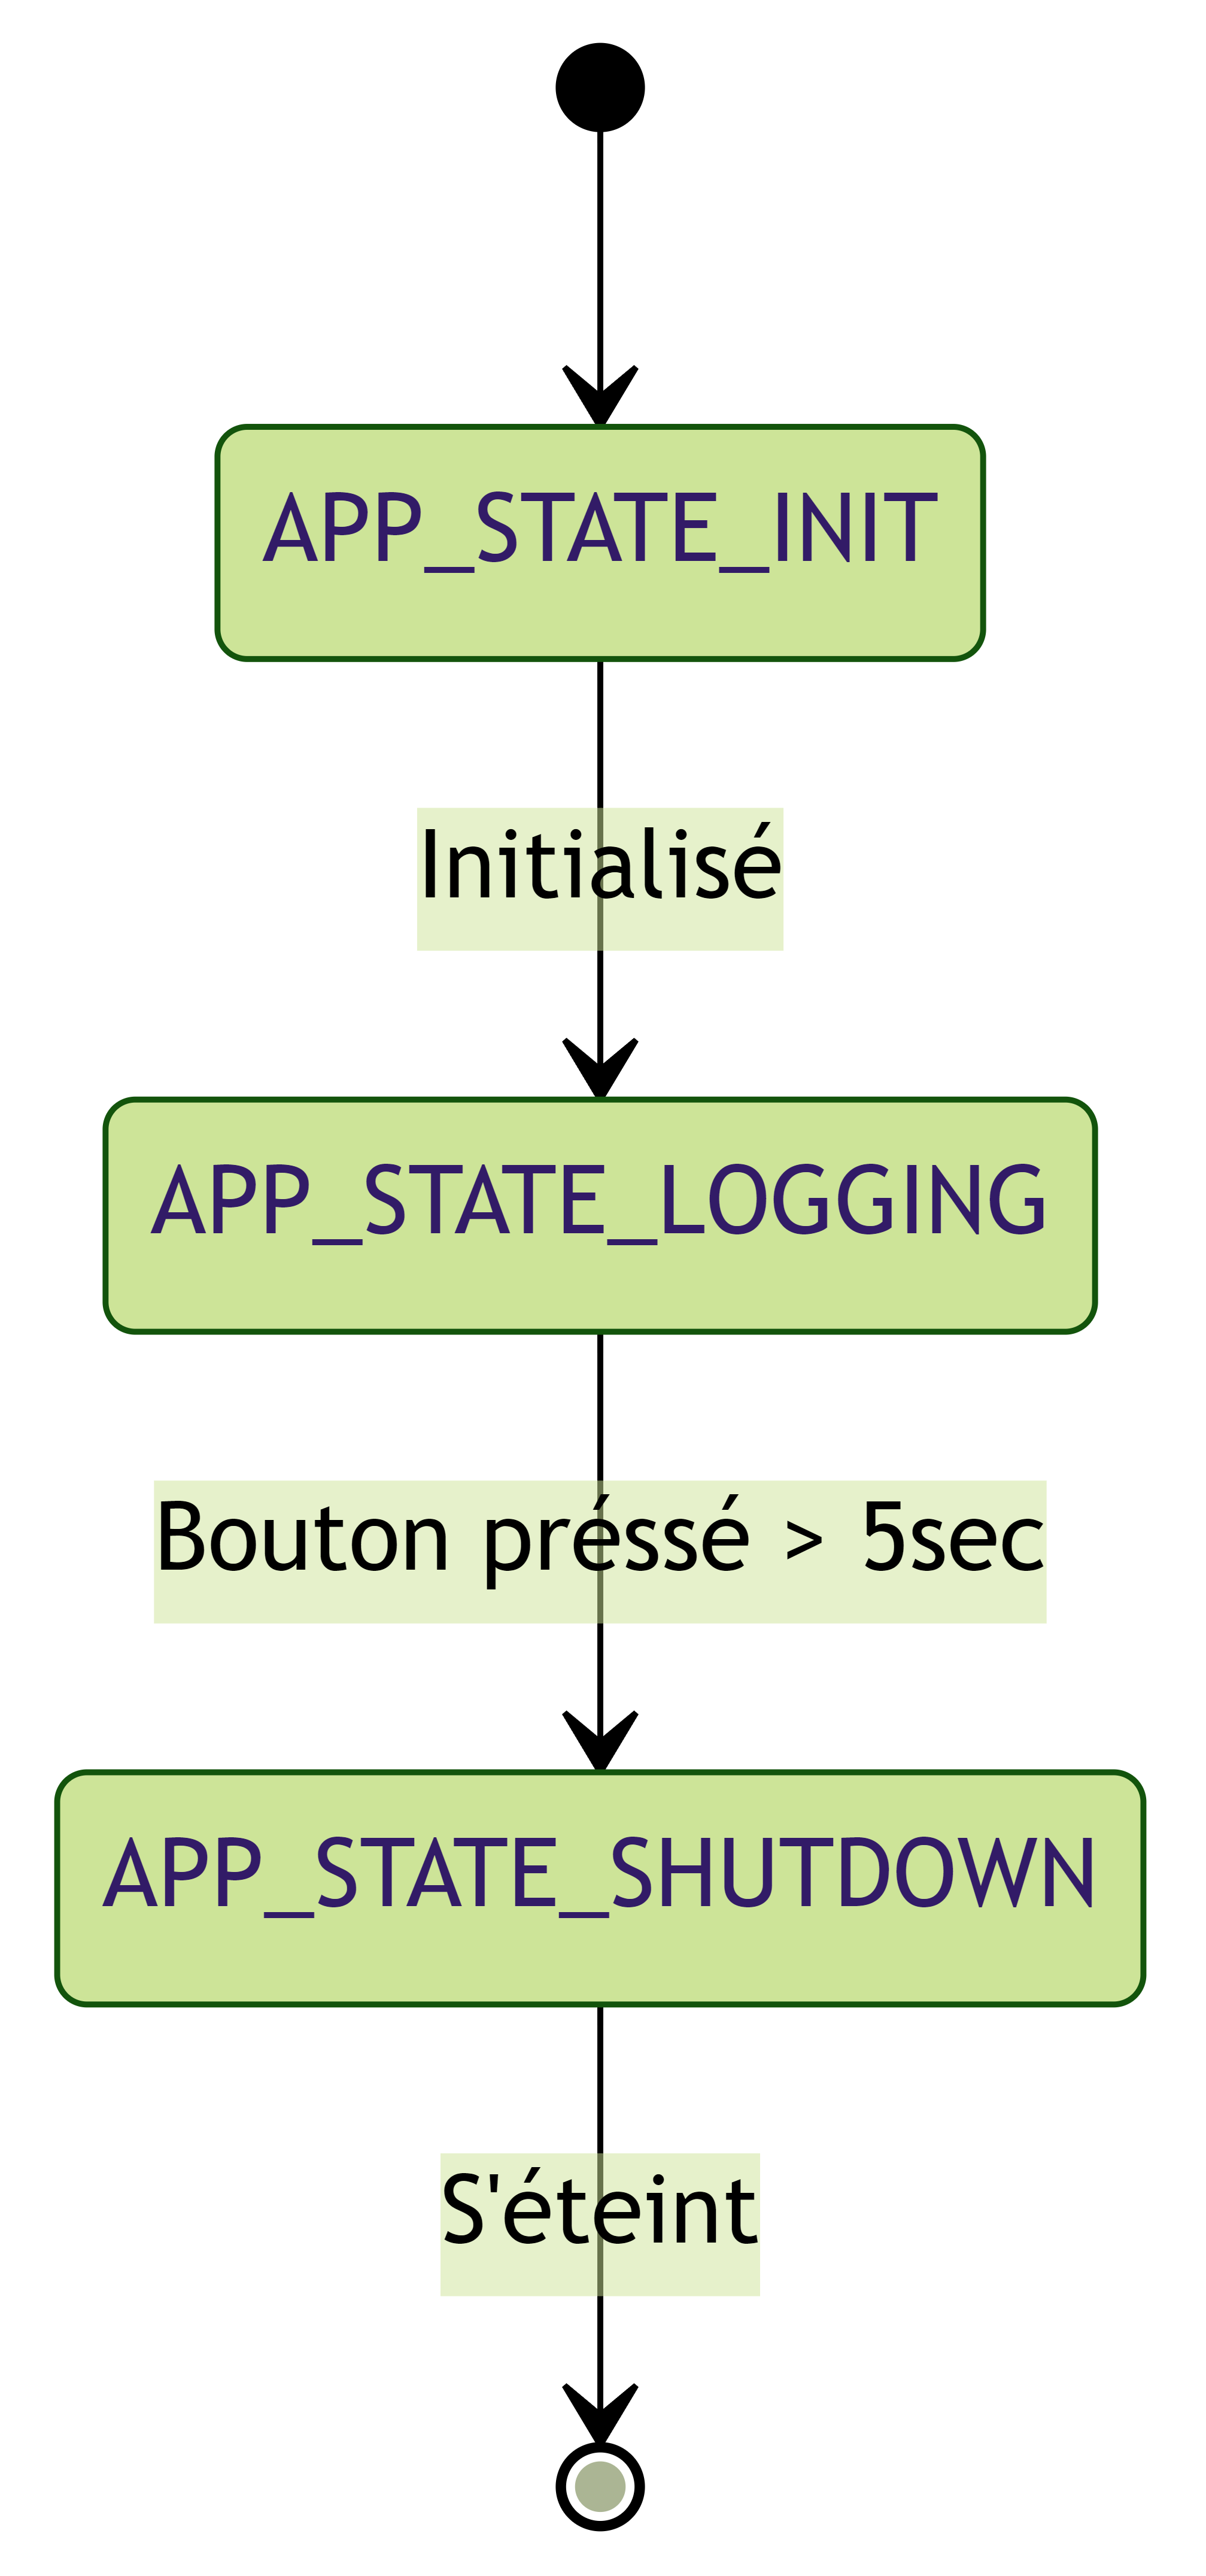
\includegraphics[width=0.28\linewidth]{Figures/Dev-SOFT/StateApp}
		\caption{Machine d'état application}
		\label{fig:stateapp}
	\end{figure}

	\clearpage
	
	\paragraph{Fonctionnement APP\_STATE\_LOGGING :} Une fois que l'application est en mode logging, le fonctionnement est décris sur la figure \ref{fig:appstatelogging} sous forme de flowchart.
	
	\begin{figure}[h]
		\centering
		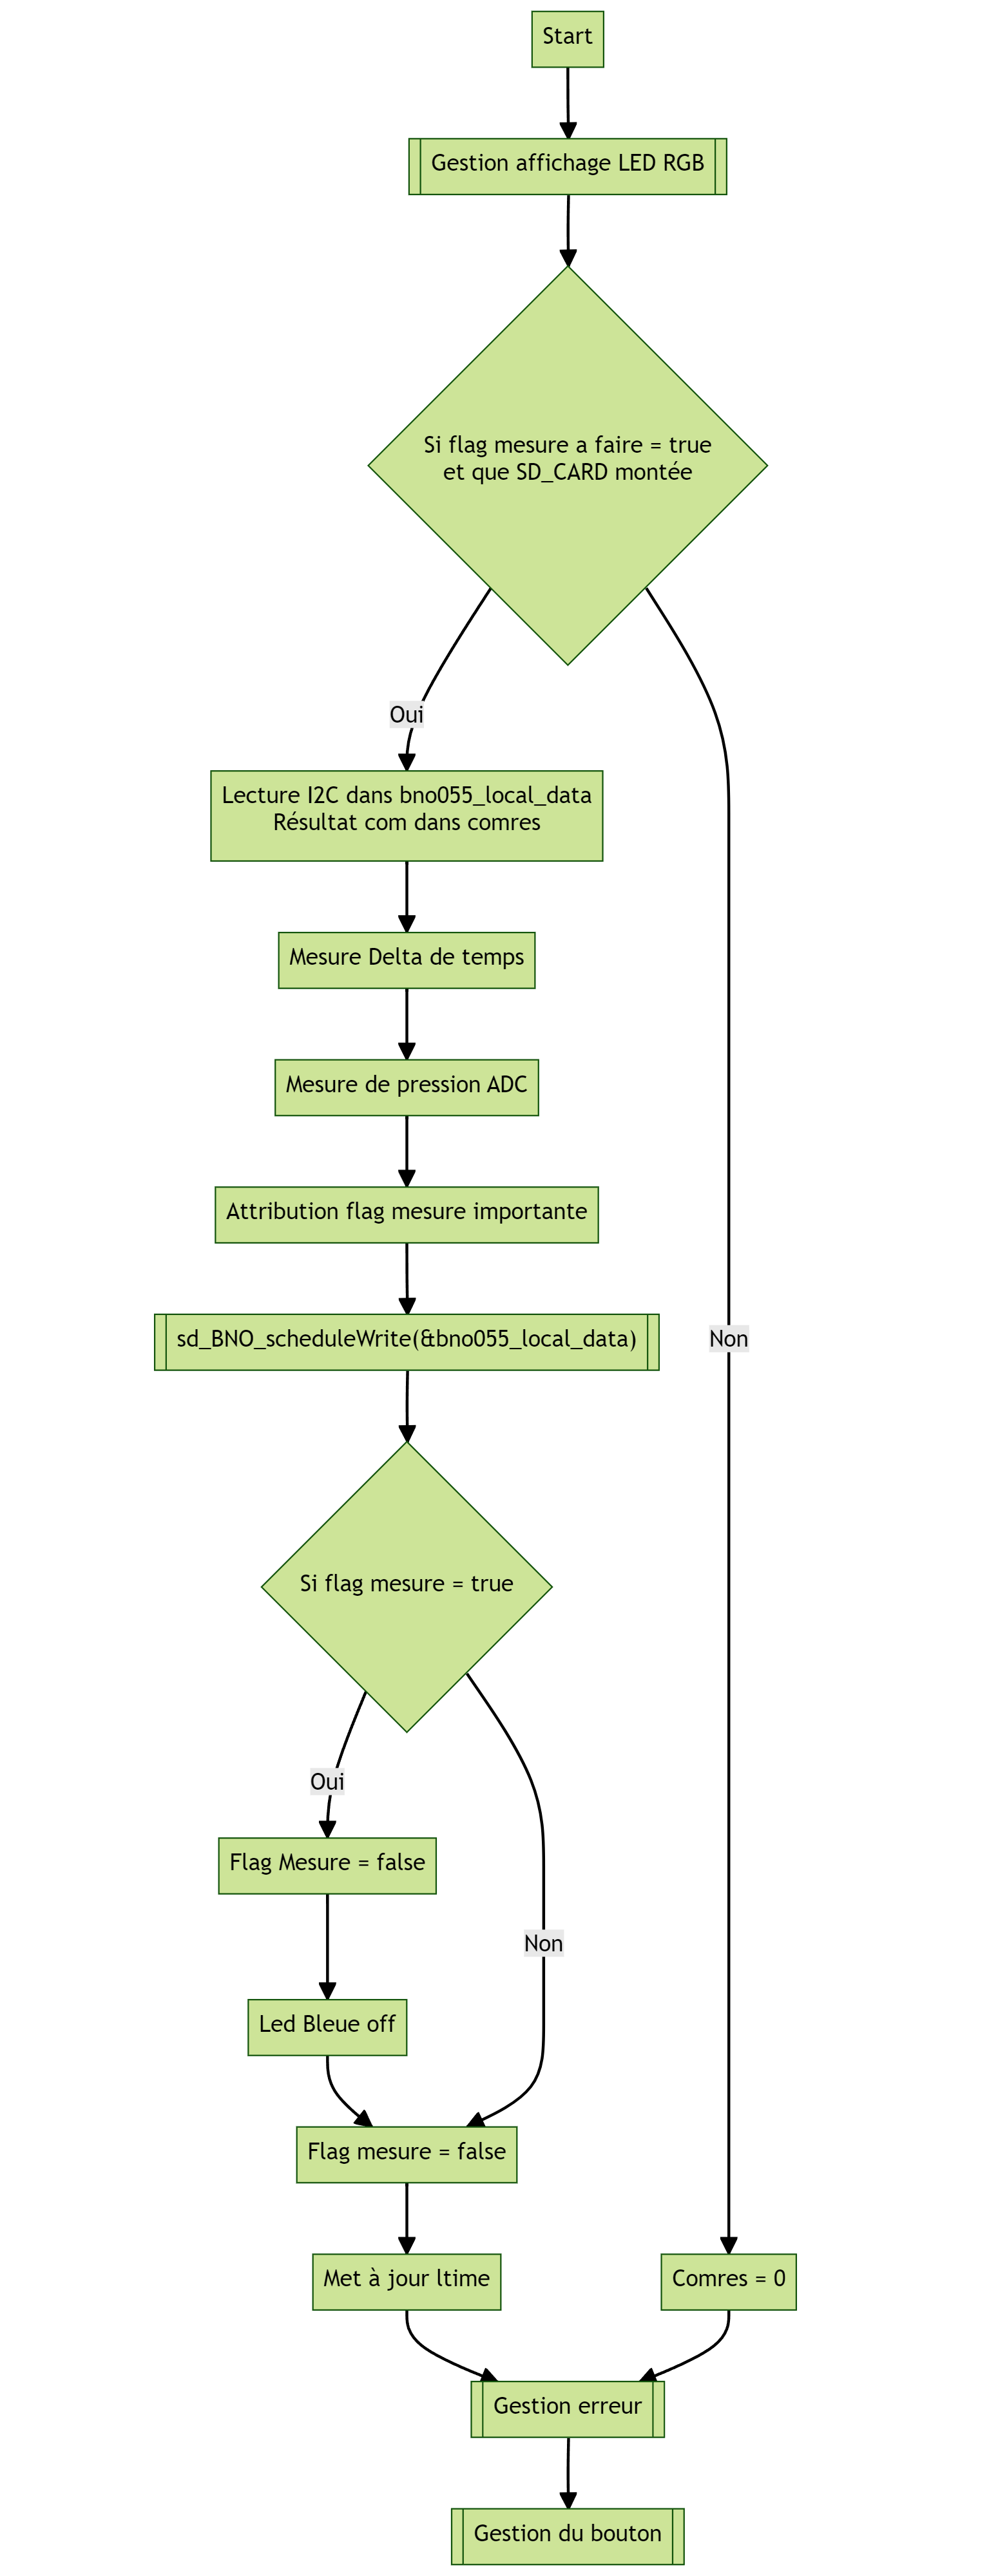
\includegraphics[width=0.446\linewidth]{Figures/Dev-SOFT/app_state_logging}
		\caption{Fowchart state logging}
		\label{fig:appstatelogging}
	\end{figure}

	\clearpage
	

}
